% shared-layout-id: ffea0a3de870bfbd233dd42ff146ecef5e3613c569500425e55a94ea70bafa66
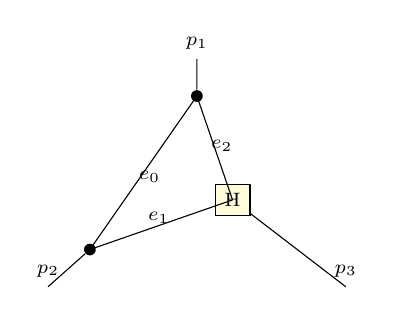
\begin{tikzpicture}[scale=.65,every node/.style={font=\scriptsize}]
\node[circle,fill,inner sep=1.5pt] (v0) at (3.27272727,4.18181818) {};
\node[circle,fill,inner sep=1.5pt] (v1) at (1.18181818,1.18181818) {};
\node[rectangle,draw,fill=yellow!15] (v2) at (3.96969697,2.15151515) {H};
\draw[black] (3.27272727,4.18181818) .. controls (2.57575758,3.18181818) and (1.87878788,2.18181818) .. (1.18181818,1.18181818);
\node at (2.34660337,2.59864834) {$e_{0}$};
\draw[black] (1.18181818,1.18181818) .. controls (2.11111111,1.50505051) and (3.04040404,1.82828283) .. (3.96969697,2.15151515);
\node at (2.52797276,1.80404802) {$e_{1}$};
\draw[black] (3.27272727,4.18181818) .. controls (3.50505051,3.50505051) and (3.73737374,2.82828283) .. (3.96969697,2.15151515);
\node at (3.75878625,3.21389361) {$e_{2}$};
\draw (v0) -- (3.27272727,4.90909091) node[above] {$p_{1}$};
\draw (v1) -- (0.36363636,0.45454545) node[above] {$p_{2}$};
\draw (v2) -- (6.18181818,0.45454545) node[above] {$p_{3}$};
\end{tikzpicture}